%%
%% This is file `sample-sigconf.tex',
%% generated with the docstrip utility.
%%
%% The original source files were:
%%
%% samples.dtx  (with options: `sigconf')
%% 
%% IMPORTANT NOTICE:
%% 
%% For the copyright see the source file.
%% 
%% Any modified versions of this file must be renamed
%% with new filenames distinct from sample-sigconf.tex.
%% 
%% For distribution of the original source see the terms
%% for copying and modification in the file samples.dtx.
%% 
%% This generated file may be distributed as long as the
%% original source files, as listed above, are part of the
%% same distribution. (The sources need not necessarily be
%% in the same archive or directory.)
%%
%% The first command in your LaTeX source must be the \documentclass command.
\documentclass[sigconf, nonacm, natbib, screen, balance=False]{acmart}

% Documentation for packages
% - ACM Article Template
%    https://www.acm.org/publications/proceedings-template
% - Pseudocode typesetting CLRS-style:
%    https://www.cs.dartmouth.edu/~thc/clrscode/clrscode3e.pdf
% - Python code typesetting
%    http://ctan.uib.no/macros/latex/contrib/listings/listings.pdf
% - AMS Math
%    http://ctan.uib.no/macros/latex/required/amsmath/amsldoc.pdf
% - Graphics
%    http://ctan.uib.no/macros/latex/required/graphics/grfguide.pdf

\usepackage{clrscode3e}  
\usepackage{listings}
\lstset{language=Python, basicstyle=\ttfamily}
\usepackage{titlesec}
\usepackage{enumitem}
\usepackage{blindtext}
\usepackage{amsmath}
\usepackage[export]{adjustbox}
\usepackage[caption=false]{subfig}
% based on https://tex.stackexchange.com/questions/279240/float-for-lstlisting
\usepackage{float}
\floatstyle{ruled}
\newfloat{listing}{tbph}{lop}
\floatname{listing}{Listing}
\def\lstfloatautorefname{Listing} % needed for hyperref/auroref

\titleformat*{\subsection}{\Large\bfseries}
\titleformat*{\subsubsection}{\large\bfseries}

\citestyle{acmauthoryear}
\newcommand{\floor}[1]{\left\lfloor #1 \right\rfloor}

%% end of the preamble, start of the body of the document source.
\begin{document}

%%
%% The "title" command has an optional parameter,
%% allowing the author to define a "short title" to be used in page headers.
\title{Mining Text Data Using Recurrent Neural Networks}
\subtitle{Data Science Report, NMBU, Spring 2021}

\author{Mohamed Radwan}
\email{mohamed.radwan@nmbu.no}
\affiliation{}  % separates Jane's and Joe's author block


%% The abstract is a short summary of the work to be presented in the
%% article.
\begin{abstract}
In this report, we will apply named entity recognition on the Groningen Meaning Bank (GMB) corpus \citep{Bos2017GMB}. We will use the Long Short Term Memory (LSTM) neural network architecture for Named Entity Recognition (NER). Application of LSTM on this dataset gave a non-strict F1 score of $0.9633$ on test data and strict F1 score of $0.793$. By customizing the embedding layer in the network through adding pretrained weights into the embedding, the non-strict F1 score improved slightly and reached $0.9695$ and the strict F1 score is $0.810$. The increase in strict F1 score is around $0.017$ and it gives us an impression that GloVe has better representation of the words in the data. This means that the embedding model GloVe is slightly more accurate than the vectors that are being trained within the used model. 

\end{abstract}
%%
%% This command processes the author and affiliation and title
%% information and builds the first part of the formatted document.
\maketitle
\section{Introduction}\label{sec:intro}
Data exists in different format and structures. In terms of structuring, data is categorized into structured and unstructured. Structured data is highly organized with clearly defined data types and is easily understood by machines. On the other hand, unstructured data (i.e., text data and images) is the type of data that don't follow an organized format. This makes the analysis of text data more challenging. Text mining is an Artificial Intelligence (AI) method and is used to extract structured meaning from this unstructured text data. Text Mining is mentioned for the first time in \citet{Feldman1998TextMA}. According to \citet{Hotho2005ABS}, Text mining involves three perspectives: information extraction, data mining, and Knowledge Discovery in Databases. In this report, we focus in Information extraction perspective. Information extraction is viewed as the process where we know in advance what kind of features we want to extract from text. According to \citet{Hotho2005ABS}, "The task of information extraction naturally decomposes into a series of processing steps, typically including tokenization, sentence segmentation, part-of-speech tagging, and the identification of named entities".
\hfill\\
Text mining employs machine learning to automate the analysis of the text data. Recurrent Neural Networks (RNNs) are specific neural network architecture that is particularly suited for sequence and text data \citep{Rumelhart:1986we}. 
\hfill\\
Named Entity Recognition is a critical step in many applications such as question answering (QA), information extraction and building chatbot systems. Extracting entities from text is helpful in identification of the key elements in a text such as the names of persons, organisations and geographical entities. For a large amount of data, extracting those entities aims to detect the most important information in the text. In other words, extracting entities helps in reducing the text into fewer features. In this report, we aim to use RNNs to extract entities from text. In Section ~\ref{sec:theory}, we will explain the theoretical details behind the the methods. In Section ~\ref{sec:methods}, we explain the workflow we use in this study. In Section.~\ref{sec:results}, the numerical results and observations are explained in details supported by figures. In Section ~\ref{sec:discu}, we use our findings and combine our observed results with explanations. 

\section{Theory}\label{sec:theory}
Recurrent neural networks or RNNs \citep{Rumelhart:1986we} are suitable to process text data because they can leverage the order of the items in the sequence. In other words, RNNs can be seen that it has memory to the items in the sequence. RNNs is multiple copies of a hidden units ($h^{t-1}, h^{t}, h^{t+1}...etc.$), as shown in Figure \ref{fig:RNN_definiton}, and each copy is passing information to its successor. This way of passing information along is what makes RNNs powerful in capturing the relationship between the elements of sequences. In RNNs, the hidden layer, as shown in Figure \ref{fig:RNN_definiton}, receives its input from both the input layer of the current time step $x^{(t)}$ and the hidden layer from the previous time step $h^{(t-1)}$. The flow of information in adjacent time steps in the hidden layer allows the network to have a memory of past events. This flow of information is usually displayed as a loop, also known as a recurrent edge which can be unfolded (figure \ref{fig:RNN_definiton}). The hidden unit $h^{(t)}$ takes input data item $x^{(t)}$ in addition to the output of previous time step $h^{(t-1)}$

\begin{figure}
  \centering
  \includegraphics[width=84mm, frame]{../figures/_rnn_definition.png}
  % figure captions below figure
  \caption{Single hidden layer RNN. The units $\big( h^{(t-1)}, h^{(t-1)}, h^{(t+1)} \dots \big)$ represent the the hidden units at different time steps while $\big( x^{(t-1)}, x^{(t-1)}, x^{(t+1)} \dots \big)$ represent the items in the input sequence at different time steps. Source: \citep{raschka2019python}}
  \label{fig:RNN_definiton}
\end{figure}
\hfill\\
There are several types of RNNs based on the shapes of inputs and outputs as shown in figure ~\ref{fig:rnns_types}. Many-to-one RNN is used when the output is a label such as sentiment analysis. One-to-many RNN are used to extract sequences from one input. Image captioning is an example of a one-to-many architecture where the input image is a single non-sequential data point and output is generated text \citep{Vinyals2015ShowAT}. Many-to-many architecture is used when both the input and output are sequences. Many-to-many architecture can be subdivided based on whether the input and output are synchronized. An example of a synchronized many-to-many task is video frame-by-frame image classification. An example of a delayed or asynchronized many-to-many modeling task would be machine translation where the input sentence must be entirely processed before its translation is produced (See Figure ~\ref{fig:rnns_types}).
\begin{figure}[ht]
  \centering
  \includegraphics[width=84mm, frame]{../figures/_rnns.png}
  % figure captions below figure
  \caption{Main architectures of RNNs. Source:\citep{raschka2019python}}
  \label{fig:rnns_types}
\end{figure}
\hfill\\
\subsection{Vanishing and Exploding Gradient}
An interesting and challenging problem with training RNNs on long sequences is what is known as vanishing and exploding gradient \citep{Pascanu2013OnTD}. This problem occurs when the absolute value of the recurrent connection weight becomes less than $1$ or greater than $1$ as shown in figure \ref{fig:vanishing}.    

\begin{figure}
  \centering
  \includegraphics[width=84mm, frame]{../figures/_vanishing.png}
  % figure captions below figure
  \caption{Vanishing and exploding gradient. $W_{hh}$ is the recurrent connection weight. Source: \citep{raschka2019python}}
  \label{fig:vanishing}
\end{figure}
\hfill\\
Essentially, the loss function does not only depends on the neurons that participated in the calculation of the output but also on the contribution of these neurons back in time. So, backpropgation of errors has to be done all the way back through time to these neurons. The full derivation of the backpropagation through time is explained in \citep{Werbos}. The loss function is dependent on the hidden units at all time steps ($1:t$). The derivative of the loss function will be:

\begin{equation}
     \frac{\partial L^{(t)}}{\partial W_{hh}} = \frac{\partial L^{(t)}}{\partial o_{t}} \times \frac{\partial o^{(t)}}{\partial h_{t}} \times \left(\sum_{k=1}^{t} \frac{\partial h^{(t)}}{\partial h^{(k)}} \times \frac{\partial h^{(k)}}{\partial W_{hh}}\right)
    \label{eq:gradientrnn}
\end{equation}
\hfill\\
where $k$ refers to the different time steps and $o_{t}$ refers to the activations of the output unit. The derivative $\frac{\partial h^{(t)}}{\partial h^{(k)}}$ is a product of adjacent time steps as shown in Eq.~\ref{eq:multipcativeunit}.

\begin{equation}
     \frac{\partial h^{(t)}}{\partial h^{(k)}} = \prod_{i = k+1}^{t}{\frac{\partial h^{(i)}}{\partial h^{(i-1)}}}  
    \label{eq:multipcativeunit}
\end{equation}
\hfill\\
In Eq.~\ref{eq:multipcativeunit}, the term is multiplied $t-k$ times. This means multiplication of the weight $W_{hh}$ by itself $t-k$ times which would result in vanishing gradient if $W_{hh}$ is less than $1$ and vanishing exploding if $W_{hh}$ is greater than $1$. One possible solution to tackle this problem is by using the Long Short-Term Memory network.   

\subsection{Long Short Term Memory}
\begin{figure}
  \centering
  \includegraphics[width=84mm, frame]{../figures/_lstm_.png}
  % figure captions below figure
  \caption{ LSTM cell architecture. The symbol $\bigodot$ is an elementwise product while the symbol $\bigoplus$ is an elementwise summation. Forget gate $f$ decides what information to delete from the memory. Input gate $i$ decides what information $\tilde{C}$ to store. Output gate $o$ decides what to output. Source: \citep{raschka2019python}}
  \label{fig:lstm_difinition}
\end{figure}
Several techniques are used to tackle the vanishing and exploding gradient problem. One of them is the Long Short-Term Memory or LSTM. LSTM is RNN architecture and was introduced by \citep{HochSchm97} and further developed by \citep{Gers1999LearningTF} and is used to capture long-term dependencies. LSTM uses gates to delete and add information from earlier states (Fig.~\ref{fig:lstm_difinition}). These gates are as follows:  

\begin{description}
\item [Forget gate] is a sigmoid function that takes in the output of the previous layer and the current layer input. The forget gate dtermines which information to keep and which information to suppress. The forget gate is shown in Eq.~\ref{eq:forgetgate}.
%
\begin{equation}
     f_t = \sigma{(W_{xf} x^{(t)}+ W_{hf}h^{(t-1)} + b_f)} 
    \label{eq:forgetgate}
\end{equation} 
%
where $W_{xf}$ and $b_{f}$ are the weights and bias between the input $x^{(t)}$ (data at time $t$) and the forget gate. $W_{hf}$ is the weight matrix between the hidden unit $h^{(t-1)}$ at time $t-1$ and the forget gate.
\hfill\\
\item [Input gate] has two branches. The first branch is a sigmoid that determines what will be updated:

\begin{equation}
     i_t = \sigma{(W_{xi} x^{(t)}+ W_{hi}h^{(t-1)} + b_i)} 
    \label{eq:inputgate1}
\end{equation} 
Here, $W_{xi}$ and $b_{i}$ are the weights and bias between the input data at time $t$ and the input gate. $W_{hi}$ is the weights matrix between the hidden unit and the input gate.
\hfill\\
The second branch is a hyperbolic tangent activation layer that outputs the candidate values that will be added to the new state:
\begin{equation}
     \tilde{C_t} = \tanh{(W_{xc} x^{(t)}+ W_{hc}h^{(t-1)} + b_c)} 
    \label{eq:inputgate2}
\end{equation} 
where $W_{xc}$ and $b_{c}$ is the weights matrix and bias between the input data at time $t$ and the candidate value. $W_{hc}$ is the weights between the hidden unit and the candidate value.
This is followed by combination of the three Eq.~\ref{eq:forgetgate}, Eq.~\ref{eq:inputgate1} and Eq.~\ref{eq:inputgate2}  from the input and forget  gates to produce the cell state $C^{(t)}$ at time $t$ as expressed as in Eq.~\ref{eq:cell_state}. Eq.~\ref{eq:cell_state} is simply an element-wise summation of what to forget from previous cell state $C^{(t-1)}$ and what to update using the candidate $\tilde{C_t}$.
\begin{equation}
     C^{(t)} = (C^{(t-1)} \odot{f_t) \oplus (i_t \odot \tilde{C_t})} 
    \label{eq:cell_state}
\end{equation} 
\hfill\\
\item [Output gate] contains two steps. The first step is a logistic sigmoid layer as expressed as:
\begin{equation}
     o_t = \sigma{(W_{xo} x^{(t)}+ W_{ho}h^{(t-1)} + b_o)} 
    \label{eq:output_gate1}
\end{equation} 
where $W_{xo}$ and $b_{o}$ are the weights and bias between the input data at time $t$ and the output gate. $W_{ho}$ is the weights between the hidden unit and the output gate.
The second step, as expressed in Eq.~\ref{eq:output_gate2}, combines $o_t$ with the internal states to obtain the output of the cell at time $t$. It is a hyperbolic tangent of the output of the second gate multiplied by the output of the first step in the output gate. The weights used in those equations are the cell memory.
\begin{equation}
     h^{(t)} = o_t \odot \tanh{(C^{(t)})} 
    \label{eq:output_gate2}
\end{equation} 
\end{description}

\hfill\\
An extension of LSTM was developed by \citet{Schuster1997BidirectionalRN} by having two LSTMs (Bidirectional LSTM or Bi-LSTM). One is responsible for the forward states (from start to end) and the other is responsible for backward states (reverse direction). This network can improve the model performance taking into account the dependence of previous sequence units on the future sequence units. 

\subsection{Word Embedding}
In order to extract features from words, words have to be encoded. One way to encode words is by one-hot-encoding \citep{ohe}, but this method will produce a large sparse matrix that is problematic in training: The feature learning process will suffer from curse of dimensionality \citep{raschka2019python}. A better way is to convert words into vectors through word embedding. Word embedding is a fundamental step for any Natural Language Processing task. Representing words as vectors, as shown in Fig.~\ref{fig:embedding}, is usually what is used to capture the relative meaning of words though their vectors representation. This means that words with similar meaning have similar representations. By clustering the words using the cosine similarity function, one can find a relative meaning of the words as shown in Fig.~\ref{fig:embedding}. Cosine similarity is a similarity measure between two vectors or the cosine of the angle between the two vectors. This embeddings matrix is used as input layer for the neural network. Several algorithms have been developed in this area like Word2Vec \citep{word2vec} and GloVe \citep{glovepaper}. 
\hfill\\
Word2Vec uses a neural network to learn these representations. The intuition behind Word2Vec is based on the assumption that the word is related to the words that surround it. So, a certain word can be trained by a log-linear classifier with goal to predict the context of the that word. Word2Vec has two approaches: Continuous Bag-of-words (CBOW) and Skip-gram (SG). CBOW approach predicts the word based on the context while SG approach predicts the context based on the word. For SG, Negative sampling method usually is used such as Skip-gram Negative Sampling (SGNS) where pairs of negative and positive samples are built and the objective is to maximize the predictions of the pairs that appear together and minimize the predictions of pairs that do not appear together. For example, if we take one word and use the above mentioned one-to-many network to predict the context from the word. Once the training is complete, there will be updated set of weights which is the embedding of that word. One important observation in Word2Vec is that Word2Vec does not take into account the frequency of co-occurance of words. 
\hfill\\
On the other hand, GloVe takes these co-occurance or frequencies into account which provide more information. GloVe algorithm is trained to aggregate word to word co-occurrence statistics in a corpus. It uses matrix factorization technique form linear algebra to measure term frequency to represent the co-occurrence matrix. Given a corpus, having $n$ words, the co-occurrence matrix will be $n \times n$ matrix where the matrix is populated with how many times word has co-occurred with other words where the vector of the word can be inferred from the context information. The authors of the GloVe , \citep{glovepaper}, propose to learn the ratios of these co-occurence probabilities. Taking two words, the dot product of two vectors equals the log of number of times the two words will occur near each other. The authors of \citep{glovepaper} explained an example: if the $P(solid|ice)$ is large and $P(solid|steam)$ is small. Therefore, the ratio of $P(solid|ice)/P(solid|steam)$ is large. The objective of the model, given a certain word, is to maximize the probability of a context to word occurrence. GloVe also makes use of CBOW and Skip-Gram similar to Word2Vec.

\begin{figure}
  \centering
  \includegraphics[width=84mm, frame]{../figures/embedding.png}
  % figure captions below figure
  \caption{General way of conversion of tokens to vectors where the embeddings can be learned through neural network. Each token is converted to vector where the distance between words is related to semantic similarity. Source: \citep{raschka2019python}}
  \label{fig:embedding}
\end{figure}

\section{Data}
The data used in this study is Groningen Meaning Bank (GMB) data that was originally developed at the University of Groningen by \citep{Bos2017GMB, gmbcorpus}. The data contains documents authored by Voice of America (VOA) with documents from the MASC dataset (\citep{Ide2008MASCTM}). 
\hfill\\
According to \citep{asheshnlp}, "This dataset is not considered a gold standard. This means that the data set is built using automatic tagging software, followed by human raters updating subsets of the data. However, this is a very large and rich data set. This data has a lot of useful annotations that make it quite suitable for training models". 
\hfill\\
The data contains $47959$ sentences and each word in the sentences is annotated as a certain entity. The vocabulary size of the data is $31817$ which represent the number of unique words in the corpus. A sample sentence is shown in Table.~\ref{tbl:sent4entites}. The data were annotated as entities according to the IOB2 annotation scheme (short for Inside, Outside and Beginning of entities). For the named entity chunks, annotation "O" represents tokens outside chunk, the annotation "B" is the beginning of a chunk while "I" marks the inside of the chunk. Also, the annotation "B" is given for a single chunk entity. The data contain $17$ unique entities as shown in Table.~\ref{tbl:entites}. The entire data is summarized in the Table.~\ref{tbl:data_summary}.

\begin{table}
  % Table captions always come *above* the table
  \caption{Text Entities in the data with their representation before the application of the IOB annotation scheme.}
  \label{tbl:entites}
  \begin{tabular}{ll}  
    \hline
    Entity & Representation \\\hline
    \verb!geo! & \verb!Geographical Entity! \\
    \verb!org! & \verb!Organization! \\
    \verb!per! & \verb!Person! \\
    \verb!gpe! & \verb!Geopolitical Entity! \\
    \verb!tim! & \verb!Time indicator! \\
    \verb!art! & \verb!Artifact! \\
    \verb!nat! & \verb!Natural Phenomenon! \\
    \verb!eve! & \verb!Event! \\\hline
  \end{tabular}
\end{table}

\begin{table}
  % Table captions always come *above* the table
  \caption{Part of sentence $4$ with labels. The sentence is "U.N. relief coordinator Jan Egeland said Sunday, U.S., Indonesian and Australian military ..."}
  \label{tbl:sent4entites}
  \begin{tabular}{ll|ll}  
    \hline
    Word & Label & Word & Label \\\hline
    \verb!U.N.! & \verb!B-geo! & \verb!,! & \verb!O! \\
    \verb!relief! & \verb!O! & \verb!U.S.! & \verb!B-geo! \\
    \verb!coordinator! & \verb!O! & \verb!,! & \verb!O! \\
    \verb!Jan! & \verb!B-per! &  \verb!Indonesian! & \verb!B-gpe!\\
    \verb!Egeland! & \verb!I-per! & \verb!and! & \verb!O! \\
    \verb!said! & \verb!O! & \verb!Australian! & \verb!B-gpe!\\
    \verb!Sunday! & \verb!B-tim! & \verb!military! & \verb!O! \\\hline
  \end{tabular}
\end{table}

\begin{table}
  % Table captions always come *above* the table
  \caption{Data Summary}
  \label{tbl:data_summary}
  \begin{tabular}{l|r}  
    \hline
    \verb!Number of unique Tokens! & \verb!31817! \\
    \verb!Number of sentences (samples)! & \verb!47959! \\
    \verb!Number of all words in data! & \verb!1048575! \\
    \verb!Maximum length of sentence! & \verb!104! \\
    \verb!Number of unique entities! & \verb!17! \\\hline
  \end{tabular}
\end{table}

\section{Methods}\label{sec:methods}
We use Python Programming Language $v3.7.9$ and Tensorflow keras API $v2.4.1$ to build the neural networks that are used in this report. Other relevant packages version are shown in Table.~\ref{tbl:packages}. The work is saved in the notebook named \verb!modeling.jpynb! with the hash \verb!20e3736d! in the GitLab repository  \url{https://gitlab.com/mhmdrdwn/datascience_report}. The models are trained under  Tesla P100 GPU with 13 GB of RAM and 16 GB of GPU RAM. 
\hfill\\
\begin{table}
  % Table captions always come *above* the table
  \caption{Used Softwares}
  \label{tbl:packages}
  \begin{tabular}{l|l}  
    \hline
    Software & Version \\\hline
    \verb!Tensorflow! & \verb!2.4.1! \\
    \verb!Numpy! & \verb!1.19.5! \\
    \verb!Pandas! & \verb!1.2.2! \\
    \verb!Seqeval! & \verb!1.2.2! \\
    \verb!ScikitLearn! & \verb!0.24.1! \\
    \verb!Seaborn! & \verb!0.11.1! \\
    \verb!Matplotlib! & \verb!3.3.3! \\\hline
  \end{tabular}
\end{table}
\hfill\\
\subsection{Tokenization}
We started by building the vocabulary of the unique words in the sentences and assign an index to each word. We use the Keras tokenizer for this process. The way the tokenizer works is that it assigns $1$ to the most common word in the text and then assigns $2$ to the second most common word until all the unique words in the text are encoded. Similarly, we build label dictionary to map each of the 17 unique tags to a unique number. Then we convert those unique numbers to a one-hot-encoded matrix where the class index is removed and a binary value, either $0$ or $1$, is inserted instead. This means that the labels vector for each training sequence is converted to $s \times 17$ matrix where $s$ is the length of the sequence and $17$ is number of labels.
\hfill\\
\subsection{Padding}
The lengths of each sentence in the data is different. The longest sentence has $104$ tokens (see Table.~\ref{tbl:data_summary}). In order to have all the sentences in the same length, we performed padding by adding zeros at the end of the each sentence until all sentences are of length $104$. 
\hfill\\
\subsection{Word Embedding}
We used two models with different methods of embedding. The first model used the Keras default embedding layer where the word representation will be learned in the network. We set the dimension of embedding to $300$. We notice that the embedding dimension has slight effect on measured metrics. This means that the vector dimension for each word is $300$ and dimension of the embedding sentence is $(104, 300)$. The second method was by using GloVe pretrained model to extract the embedding vectors of the words and then inserting these weights as initial weights for the embedding layer in the model. We use the version of GloVe that has $840$ billion unique words from \citet{glove840}. The embedding vector dimension of words in GloVe is $300$.
\hfill\\
\subsection{Building the model}
We split the data into training and testing data where the training data represent $0.8$ and testing data represent $0.2$ (testing data contains $9592$ sequences).
The used neural network architectures are as shown in tables \ref{tbl:rnn_used} and \ref{tbl:rnn_glove}. Both the models start with embedding the features followed by hidden $16$ bidirectional LSTM units. The output layer (Dense layer in Table.~\ref{tbl:rnn_used}) is a regular fully connected neural network layer with the number of labels. The number of labels is set to $18$ which represent the number of labels plus the padding zero. The loss function is categorical cross entropy (Eq.~\ref{eq:cce}). The validation data (0.1 of the train data) is chosen randomly within the Keras model to monitor the accuracy.

\begin{equation}
    CCE = - \sum_{i=1}^{C} t^{i} \log(p_{i})
    \label{eq:cce}
\end{equation} 
In Eq.~\ref{eq:cce}, $t_{i}$ and $p_{i}$ are the ground truth and the activation of the class $i$. This loss is calculated for each of the $C$ classes.
\hfill\\
The number of trainable parameters for Bidirectional LSTM and Bidirectional LSTM with GloVe are $513906$ and $9586570$ respectively. The significant increase in the number of trainable parameters is because the GloVe algorithm gives a vector of dimension $300$ for each word. The model produces a probability using Softmax activation function in the output layer.

\begin{table}
  % Table captions always come *above* the table
  \caption{Bidirectional LSTM network. The parameters of the embedding is product of ($300 \times 31817$ plus $300$ biases where $31817$ is number of unique tokens).}
  \label{tbl:rnn_used}
  \begin{tabular}{l|l|r}  
    \hline
    Layer & Output Shape & Parameters \\\hline
    \verb!Input Layer! & \verb!104! & \verb!0! \\
    \verb!Default Embedding! & \verb!(104, 300)! & \verb!9545400! \\
    \verb!Bidirectional LSTM! & \verb!(104, 128)! & \verb!186880!\\
    \verb!LSTM! & \verb!(104, 64)! & \verb!49408!\\
    \verb!Dense! & \verb!(104, 18)! & \verb!1170! \\
    \verb!Parameters! & \verb!! & \verb!9782858!  \\\hline
  \end{tabular}
\end{table}

\begin{table}
  % Table captions always come *above* the table
  \caption{Bidirectional LSTM network with Glove embedding}
  \label{tbl:rnn_glove}
  \begin{tabular}{l|l|r}  
    \hline
    Layer & Output Shape & Parameters \\\hline
    \verb!Input Layer! & \verb!104! & \verb!0! \\
    \verb!Glove Embedding! & \verb!(104, 300)! & \verb!9545400! \\
    \verb!Bidirectional LSTM! & \verb!(104, 128)! & \verb!186880!\\
    \verb!LSTM! & \verb!(104, 64)! & \verb!49408!\\
    \verb!Dense! & \verb!(104, 18)! & \verb!1170! \\
    \verb!Parameters! & \verb!! & \verb!9782858!  \\\hline
  \end{tabular}
\end{table}

\hfill\\
\subsection{Evaluation metrics}\label{sec:metrics}
We recorded Precision, Recall, F1 score \citep{Powers2008EvaluationFP} and confusion matrix to evaluate the models and to perform error analysis. Precision measures the number of positive class predictions (TP) that actually belong to the positive class:
\begin{equation}
     P = \frac{TP}{TP+FP}
    \label{eq:prec_form}
\end{equation} 
\hfill\\
On the other hand, Recall is the number of positive class predictions made out of all positive classes:
\begin{equation}
     R = \frac{TP}{TP+FN}
    \label{eq:recall_form}
\end{equation} 
\hfill\\
F1 combines both Precision and Recall in a balanced measure as:
\begin{equation}
     F1 = \frac{2 \times P \times R}{P+R}
    \label{eq:f1_form}
\end{equation} 
\hfill\\
Since we add padding zeros at the end of the sequences that will affect the measured metrics (increases metrics), we exclude the padding zeros from the calculations of all these metrics using a mask in our implementation of the metrics.
\hfill\\
For further evaluation of the models, we use the package Seqeval (see Table.~\ref{tbl:packages}) to quantify F1, Precision and Recall. Compared to the above mentioned metrics, Seqeval uses strict metrics that only quantify True Positive (TP) if the whole entity is predicted correctly \citep{seqeval}. This means that partially predicted entities do not count as TP as shown in Table.~\ref{tbl:strict}. Precision, Recall and F1 scores can be measured as per sentence (micro measure) and over the entire corpus (macro measure). The weighted measure is calculated for each label and then their average is weighted by the label support.

\begin{table}
  % Table captions always come *above* the table
  \caption{Strict Measures. Prediction $1$ is counted as one TP while Prediction $2$ is zero TP.}
  \label{tbl:strict}
  \begin{tabular}{c|c|c|c|c}  
    \hline
    &coordinator & Jan & Egeland & said \\\hline
    \verb!True! & \verb!O! & \verb!B-Per! & \verb!I-Per! & \verb!O! \\
    \verb!Prediction 1! & \verb!O! & \verb!B-Per! & \verb!I-Per! & \verb!O! \\
    \verb!Prediction 2! & \verb!O! & \verb!B-Per! & \verb!O! & \verb!O! \\\hline
  \end{tabular}
\end{table}
\hfill\\
\subsection{Hyperparameters Optimization}
We experiment manually using different combination of hyperparameters while monitoring the validation set evaluation metrics. We choose learning rate from a logarithmic scale (i.e., $0.00001$ ,$0.0001$, $0.001$, $0.01$, $0.1$). Then, we focus search further on learning rates with-in the range ($0.005$, $0.05$) which shows best results. The optimal choice is using Adam optimizer with learning rate $0.01$ which shows the highest validation scores. Regularization dropouts of $0.5$ were used in both network. This means that half of the neurons are randomly muted to reduce the complexity of the network and the overfitting according to \citep{dropout}. A full list of experimented hyperparameters are shown in Table.~\ref{tbl:hyperparameters}. Other hyperparameters such as the number of units have minimal effect on the measured metrics of the validation set.
\begin{table}. 
  % Table captions always come *above* the table
  \caption{Hyperparameters optimization choices}
  \label{tbl:hyperparameters}
  \begin{tabular}{l|l|r}  
    \hline
     & Hyperparameters Search &  Optimal Choice \\
    \hline
    Learning rates & \verb!(0.00001, 0.0001,! & \verb!0.01!\\
    & \verb! 0.001, 0.005,! \\
    & \verb! 0.008, 0.01, 0.02,! \\
    & \verb! 0.05, 0.1)! \\
    Optimizers & \verb!(Adam, RMSprop)! & \verb!Adam! \\
    Number of Units & \verb!(32 , 64, 128, 256)! & \verb!64! \\
    Dropout & \verb!(0.2, 0.3, 0.4, 0.5)! & \verb!0.5! \\\hline
  \end{tabular}
\end{table}

\section{Results}\label{sec:results}
Table \ref{tbl:results_compare} shows the comparison between the results of the two models. The resulting scores show that the two implemented model are generalizing on the validation and the testing data. Evaluating the models on the validation and testing data shows very similar values. The recorded training time for both the implemented models is approximately $205$ seconds per epoch. This means that the total duration of training each of the models is approximately $34$ minutes.   

\begin{table}
  % Table captions always come *above* the table
  \caption{Results achieved by Bidirectional LSTM (BiLSTM) and Bidirectional LSTM with Glove embedding (BiLSTM-GloVe).}
  \label{tbl:results_compare}
  \begin{tabular}{c|c|c|c}  
    \hline
    \verb!! & \verb!! & Train  & Test \\\hline
    \verb!! & \verb!Recall! & \verb!0.9634!  & \verb!0.9556! \\
    \verb!BiLSTM! & \verb!Precision!  & \verb!0.9731! & \verb!0.9634! \\
    \verb!! & \verb!F1! & \verb!0.9682!  & \verb!0.9595!\\\hline
    \verb!! & \verb!Recall! & \verb!0.9658!  & \verb!0.9598! \\
    \verb!BiLSTM-GloVe! &  \verb!Precision! & \verb!0.9745!  & \verb!0.9669! \\
    \verb!! &  \verb!F1! & \verb!0.9702! & \verb!0.9633!  \\\hline
  \end{tabular}
\end{table}

\subsection{Bidirectional LSTM}
After training for 10 epochs, bidirectional LSTM achieved F1 score of $0.9682$ on training data while the scored F1 scores on test data  $0.9595$ respectively. From Fig.~\ref{fig:f1_bilstm}, It is noticed that the validation F1 score remains almost constant around $0.9600$ after epoch number $5$ while the training score continued to increase slightly until it reaches $0.9783$ at epoch number $10$.

\begin{figure}
  \centering
  \begin{subfig}{a)}
  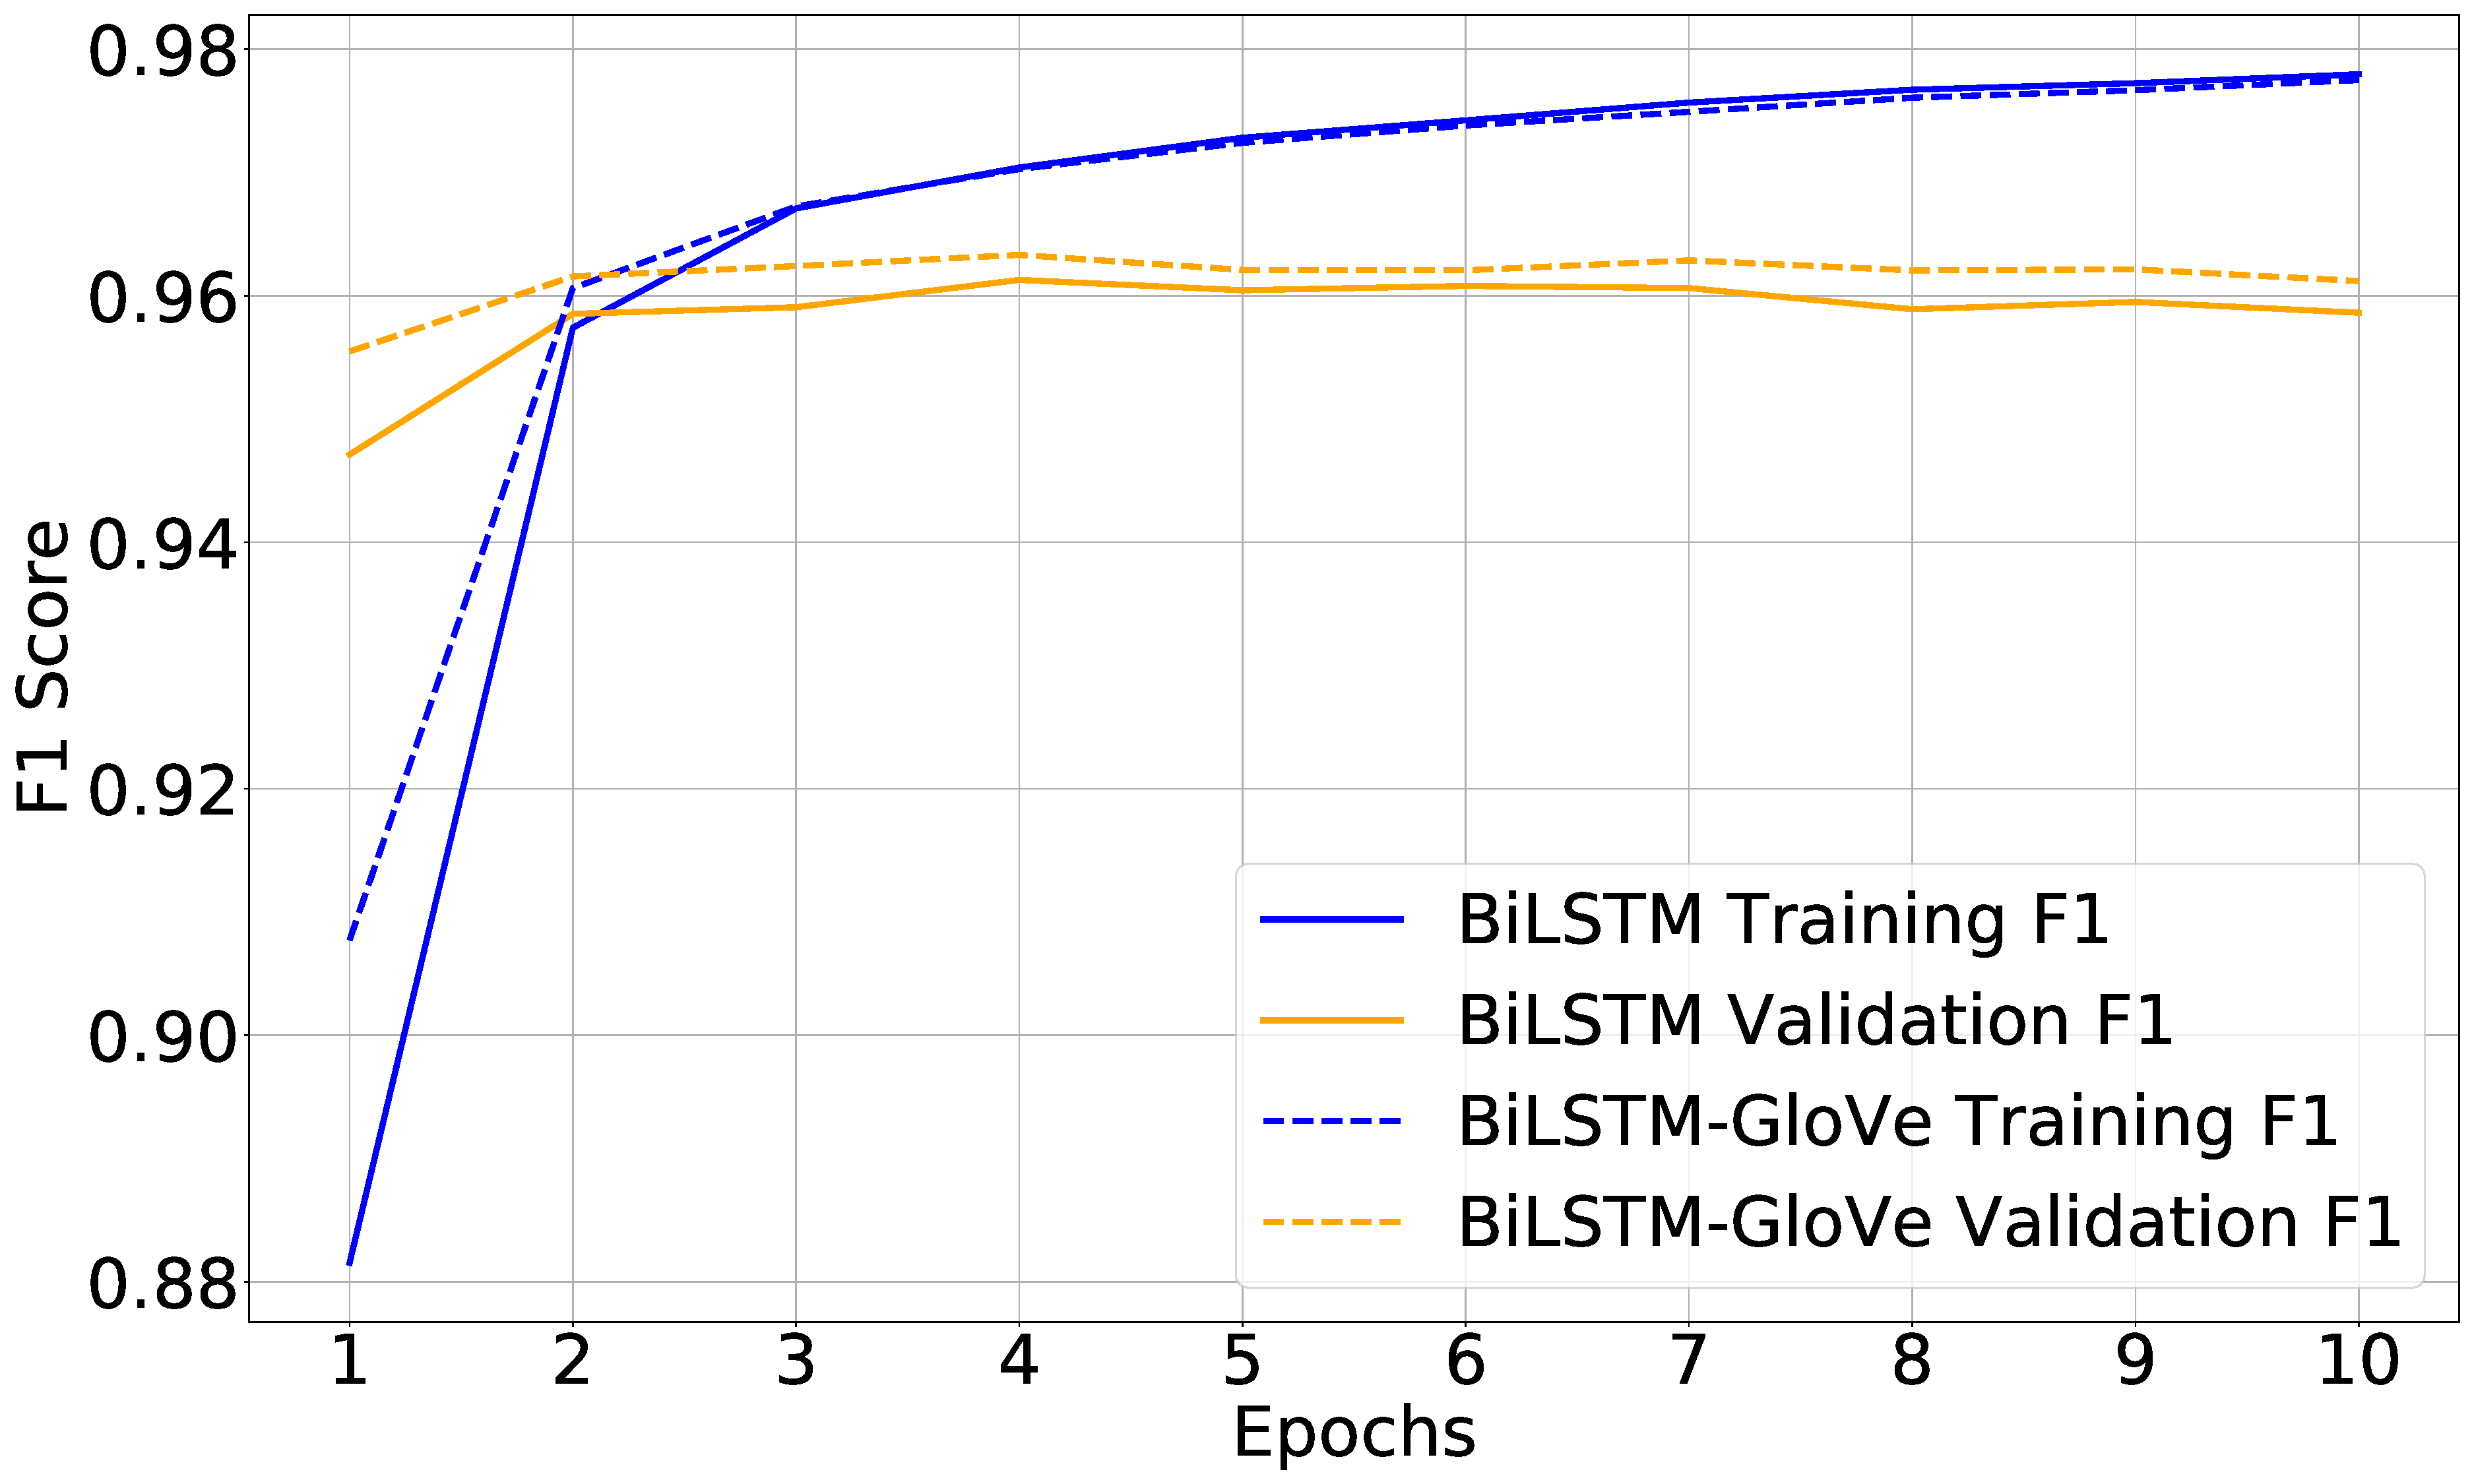
\includegraphics[width=84mm, frame]{../figures/Training_F1.pdf}
  \end{subfig}
  \begin{subfig}{b)}
  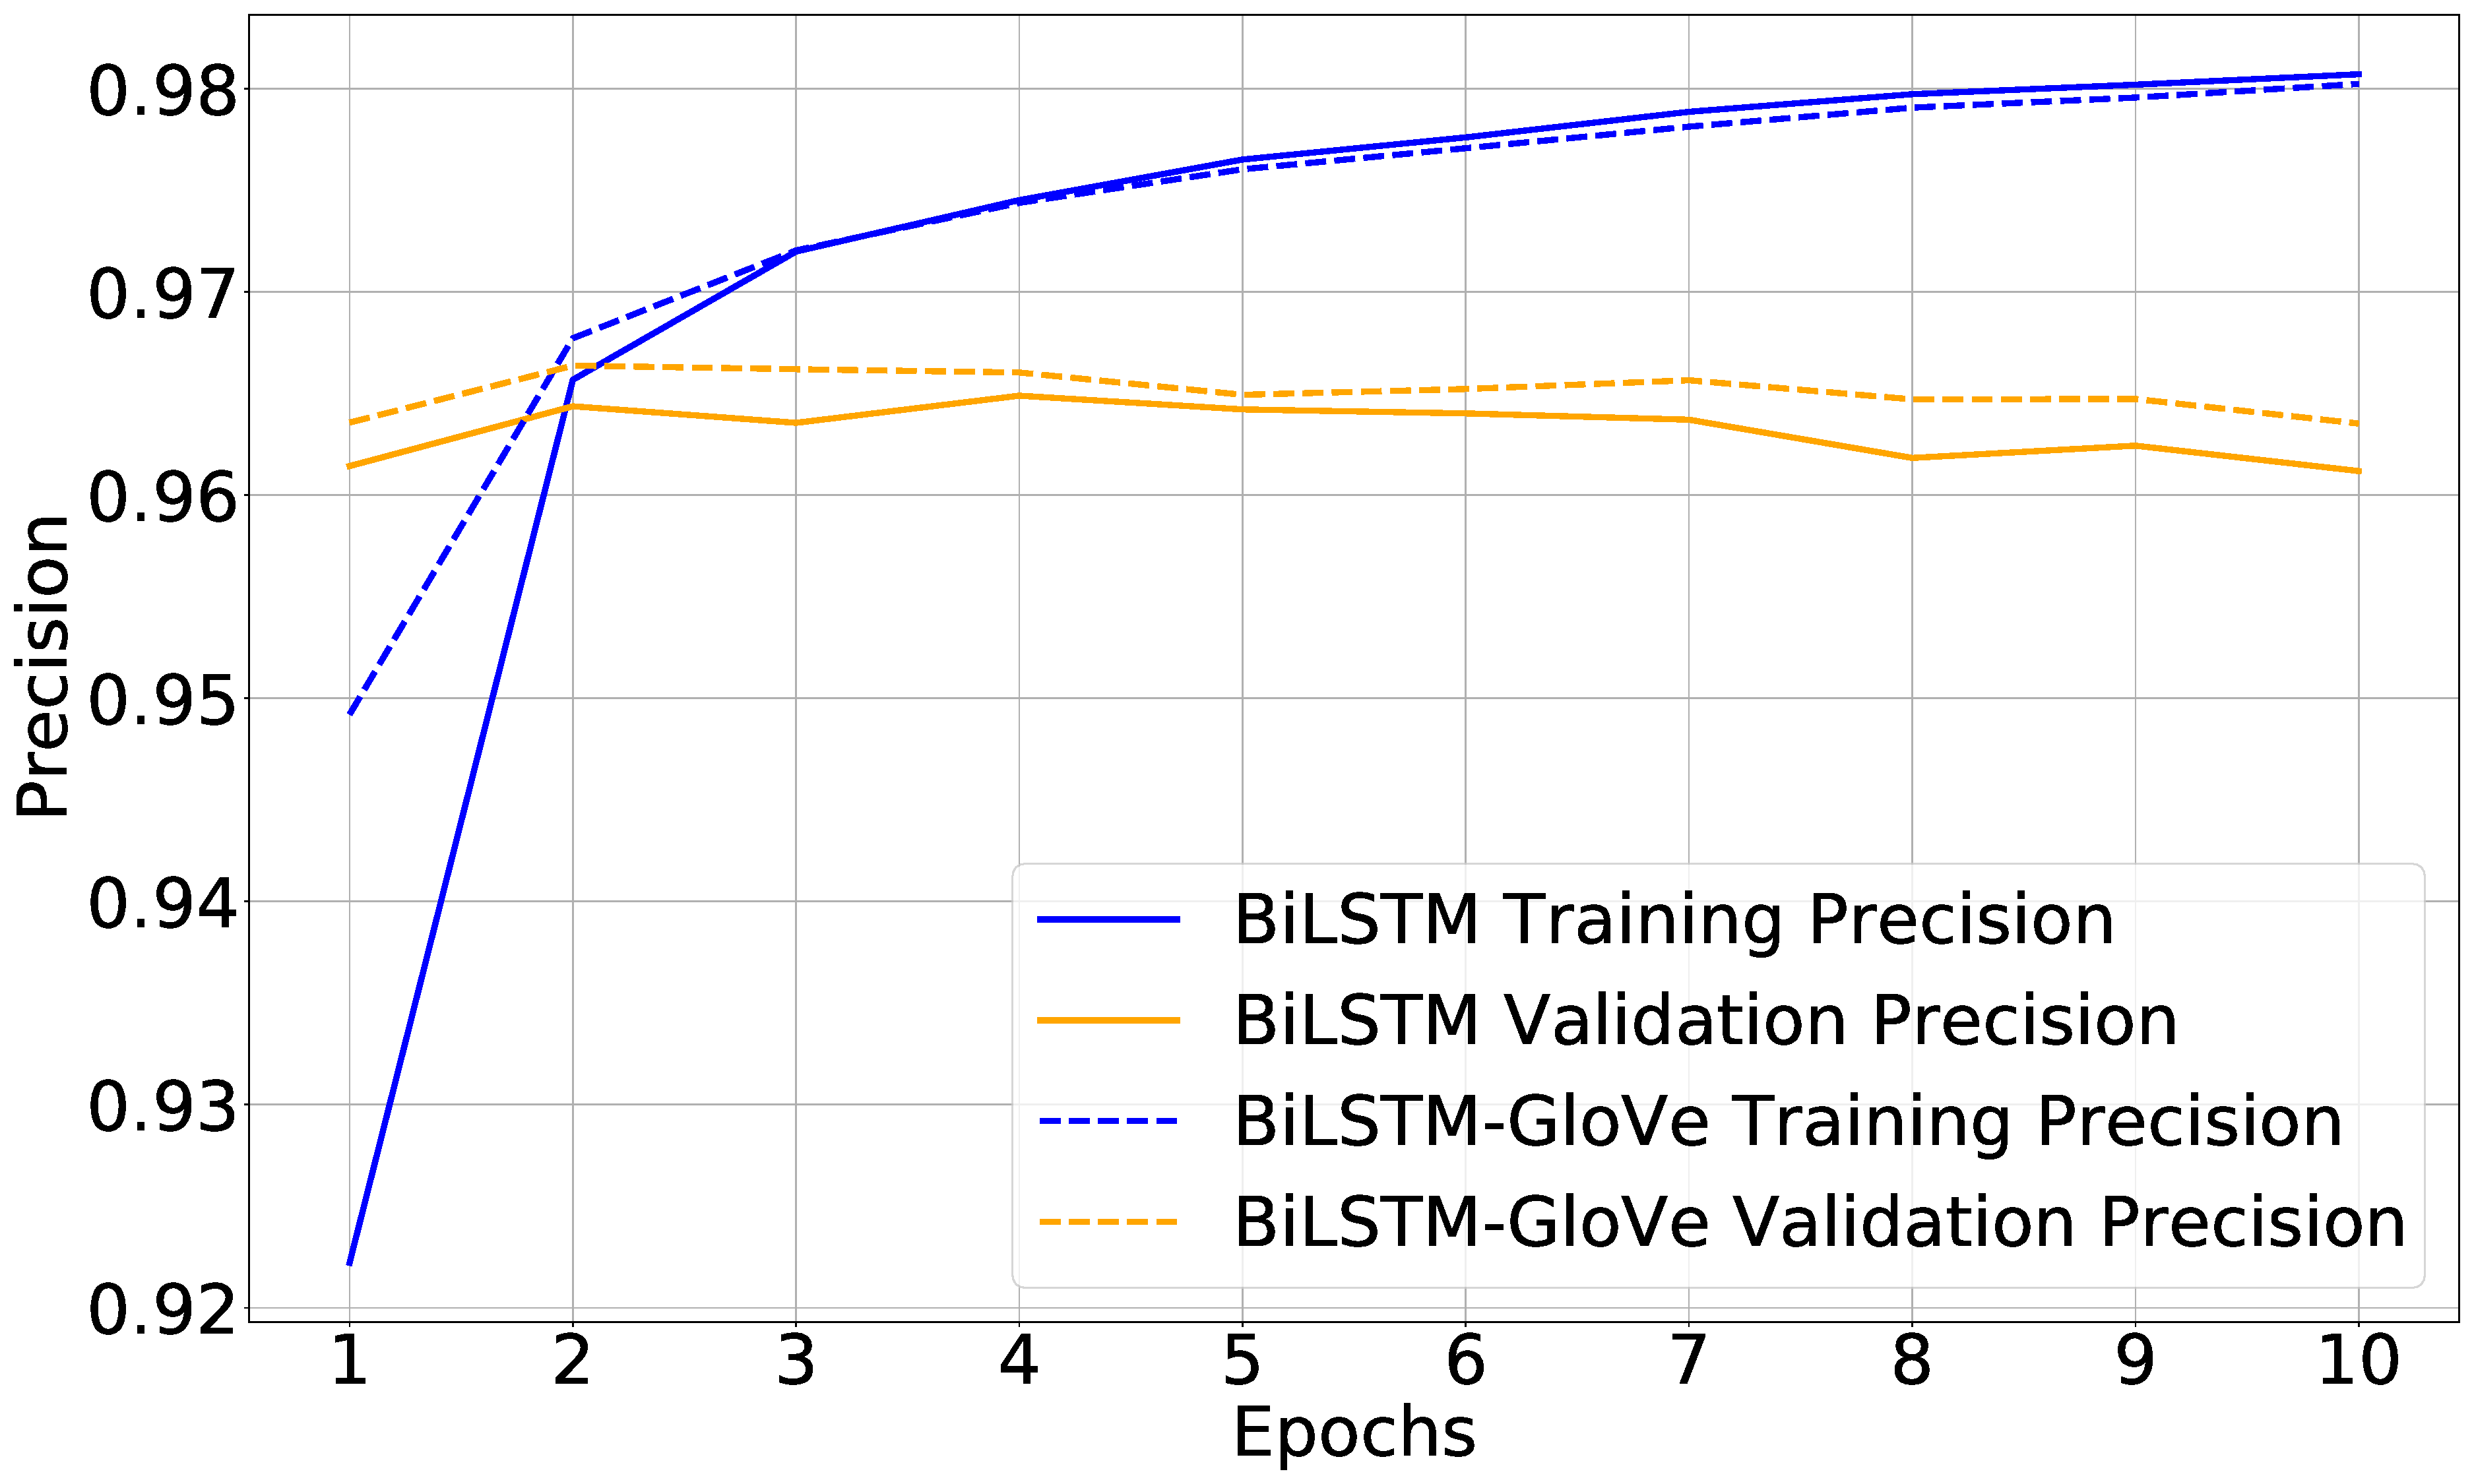
\includegraphics[width=84mm, frame]{../figures/Training_Precision.pdf}
  \end{subfig}
  \begin{subfig}{c)}
  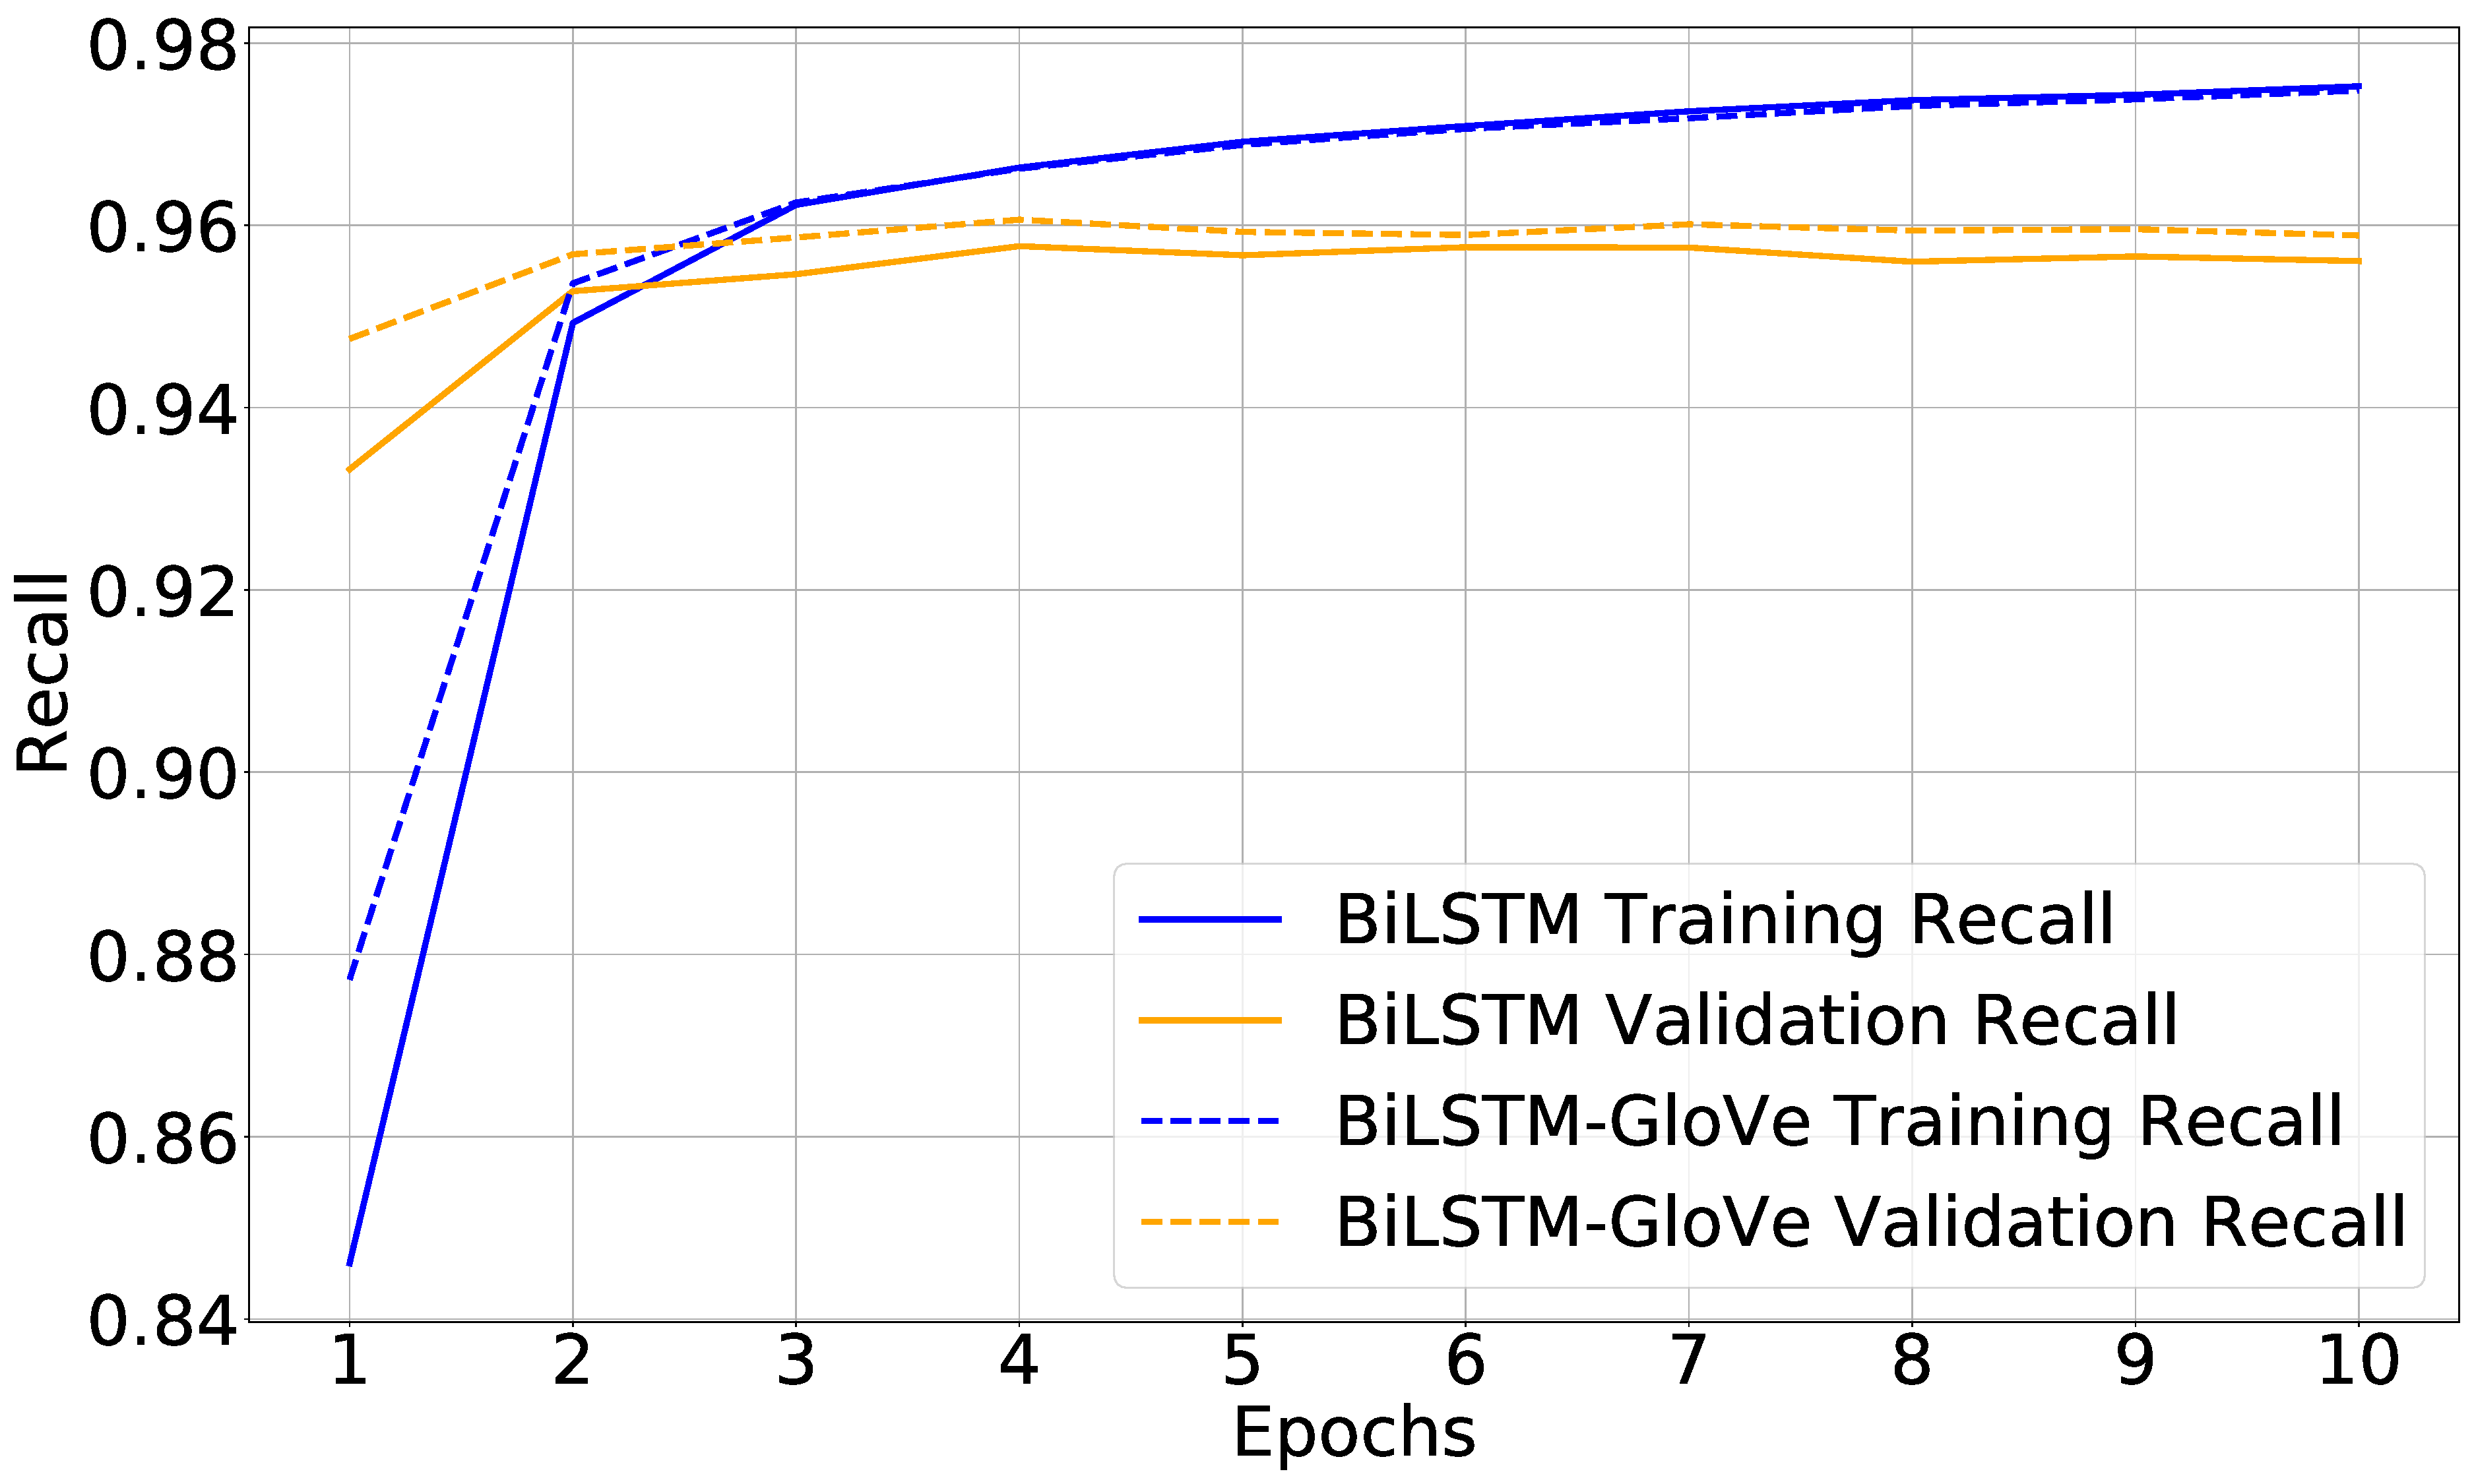
\includegraphics[width=84mm, frame]{../figures/Training_Recall.pdf}
  \end{subfig}
  % figure captions below figure
  \caption{Training and validation a) F1, b) Precision and c) Recall score using the two models.}
  \label{fig:f1_bilstm}
\end{figure}
\hfill\\
Fig.~\ref{fig:f1_bilstm} also shows the precision score achieved by bidirectional LSTM which starts at $0.9631$ and ends at $0.9605$ on validation data. Despite the change of precision score on training data from $0.8315$ to $0.9811$ after $10$ epochs, validation precision score remains almost constant. The precision score of the testing data is $0.9609$.    
\hfill\\
Fig.~\ref{fig:f1_bilstm} shows the recall score of bidirectional LSTM model. The recall score is $0.9634$, $0.9543$ and $0.9556$  on training and testing data respectively. We notice from Fig.~\ref{fig:f1_bilstm} that validation recall starts at $0.9485$ and end $0.9587$ after $10$ epochs. 
\hfill\\
Heatmap in Fig.~\ref{fig:bilstmconfusion} shows the confusion matrix between the ground truth labels and the predicted labels. The confusion matrix indicates the label 'O' or 'other' is accompanied with most of the errors in the prediction (false positive and false negative).    

\begin{figure}
  \centering
  \begin{subfig}{a)}
  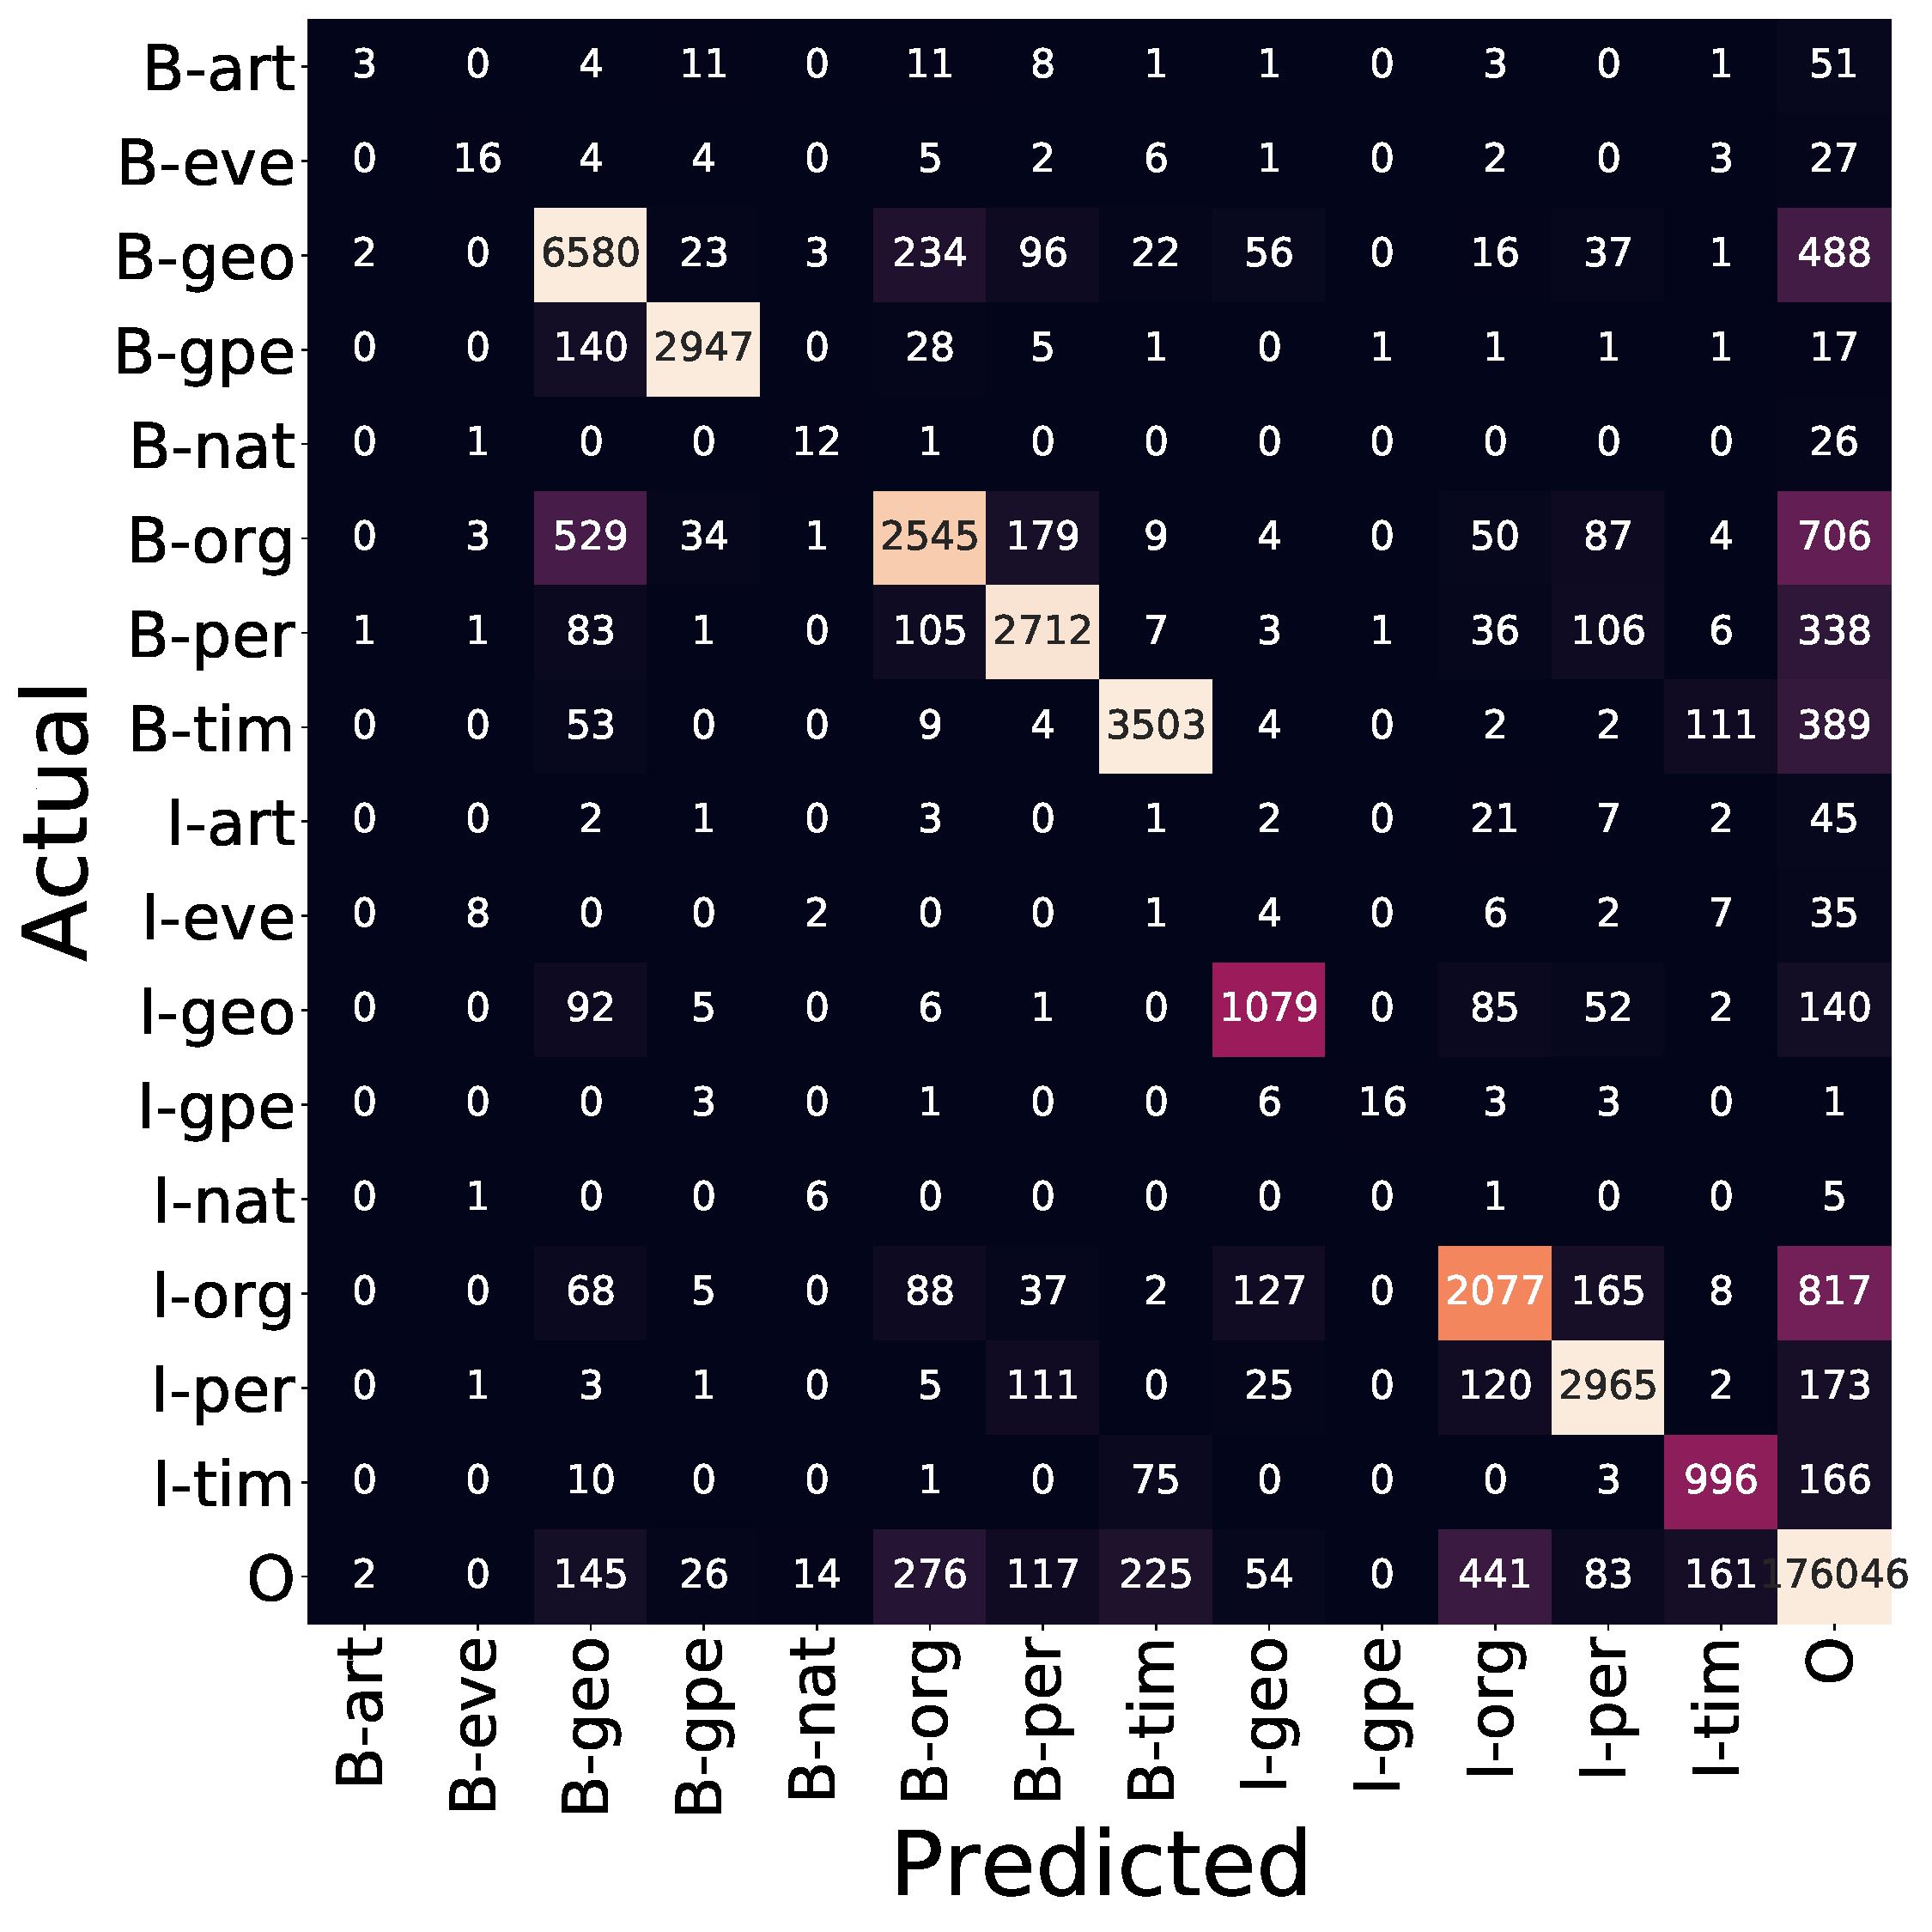
\includegraphics[width=84mm, frame]{../figures/conf_matrix.pdf}
  \end{subfig}
  \begin{subfig}{b)}
  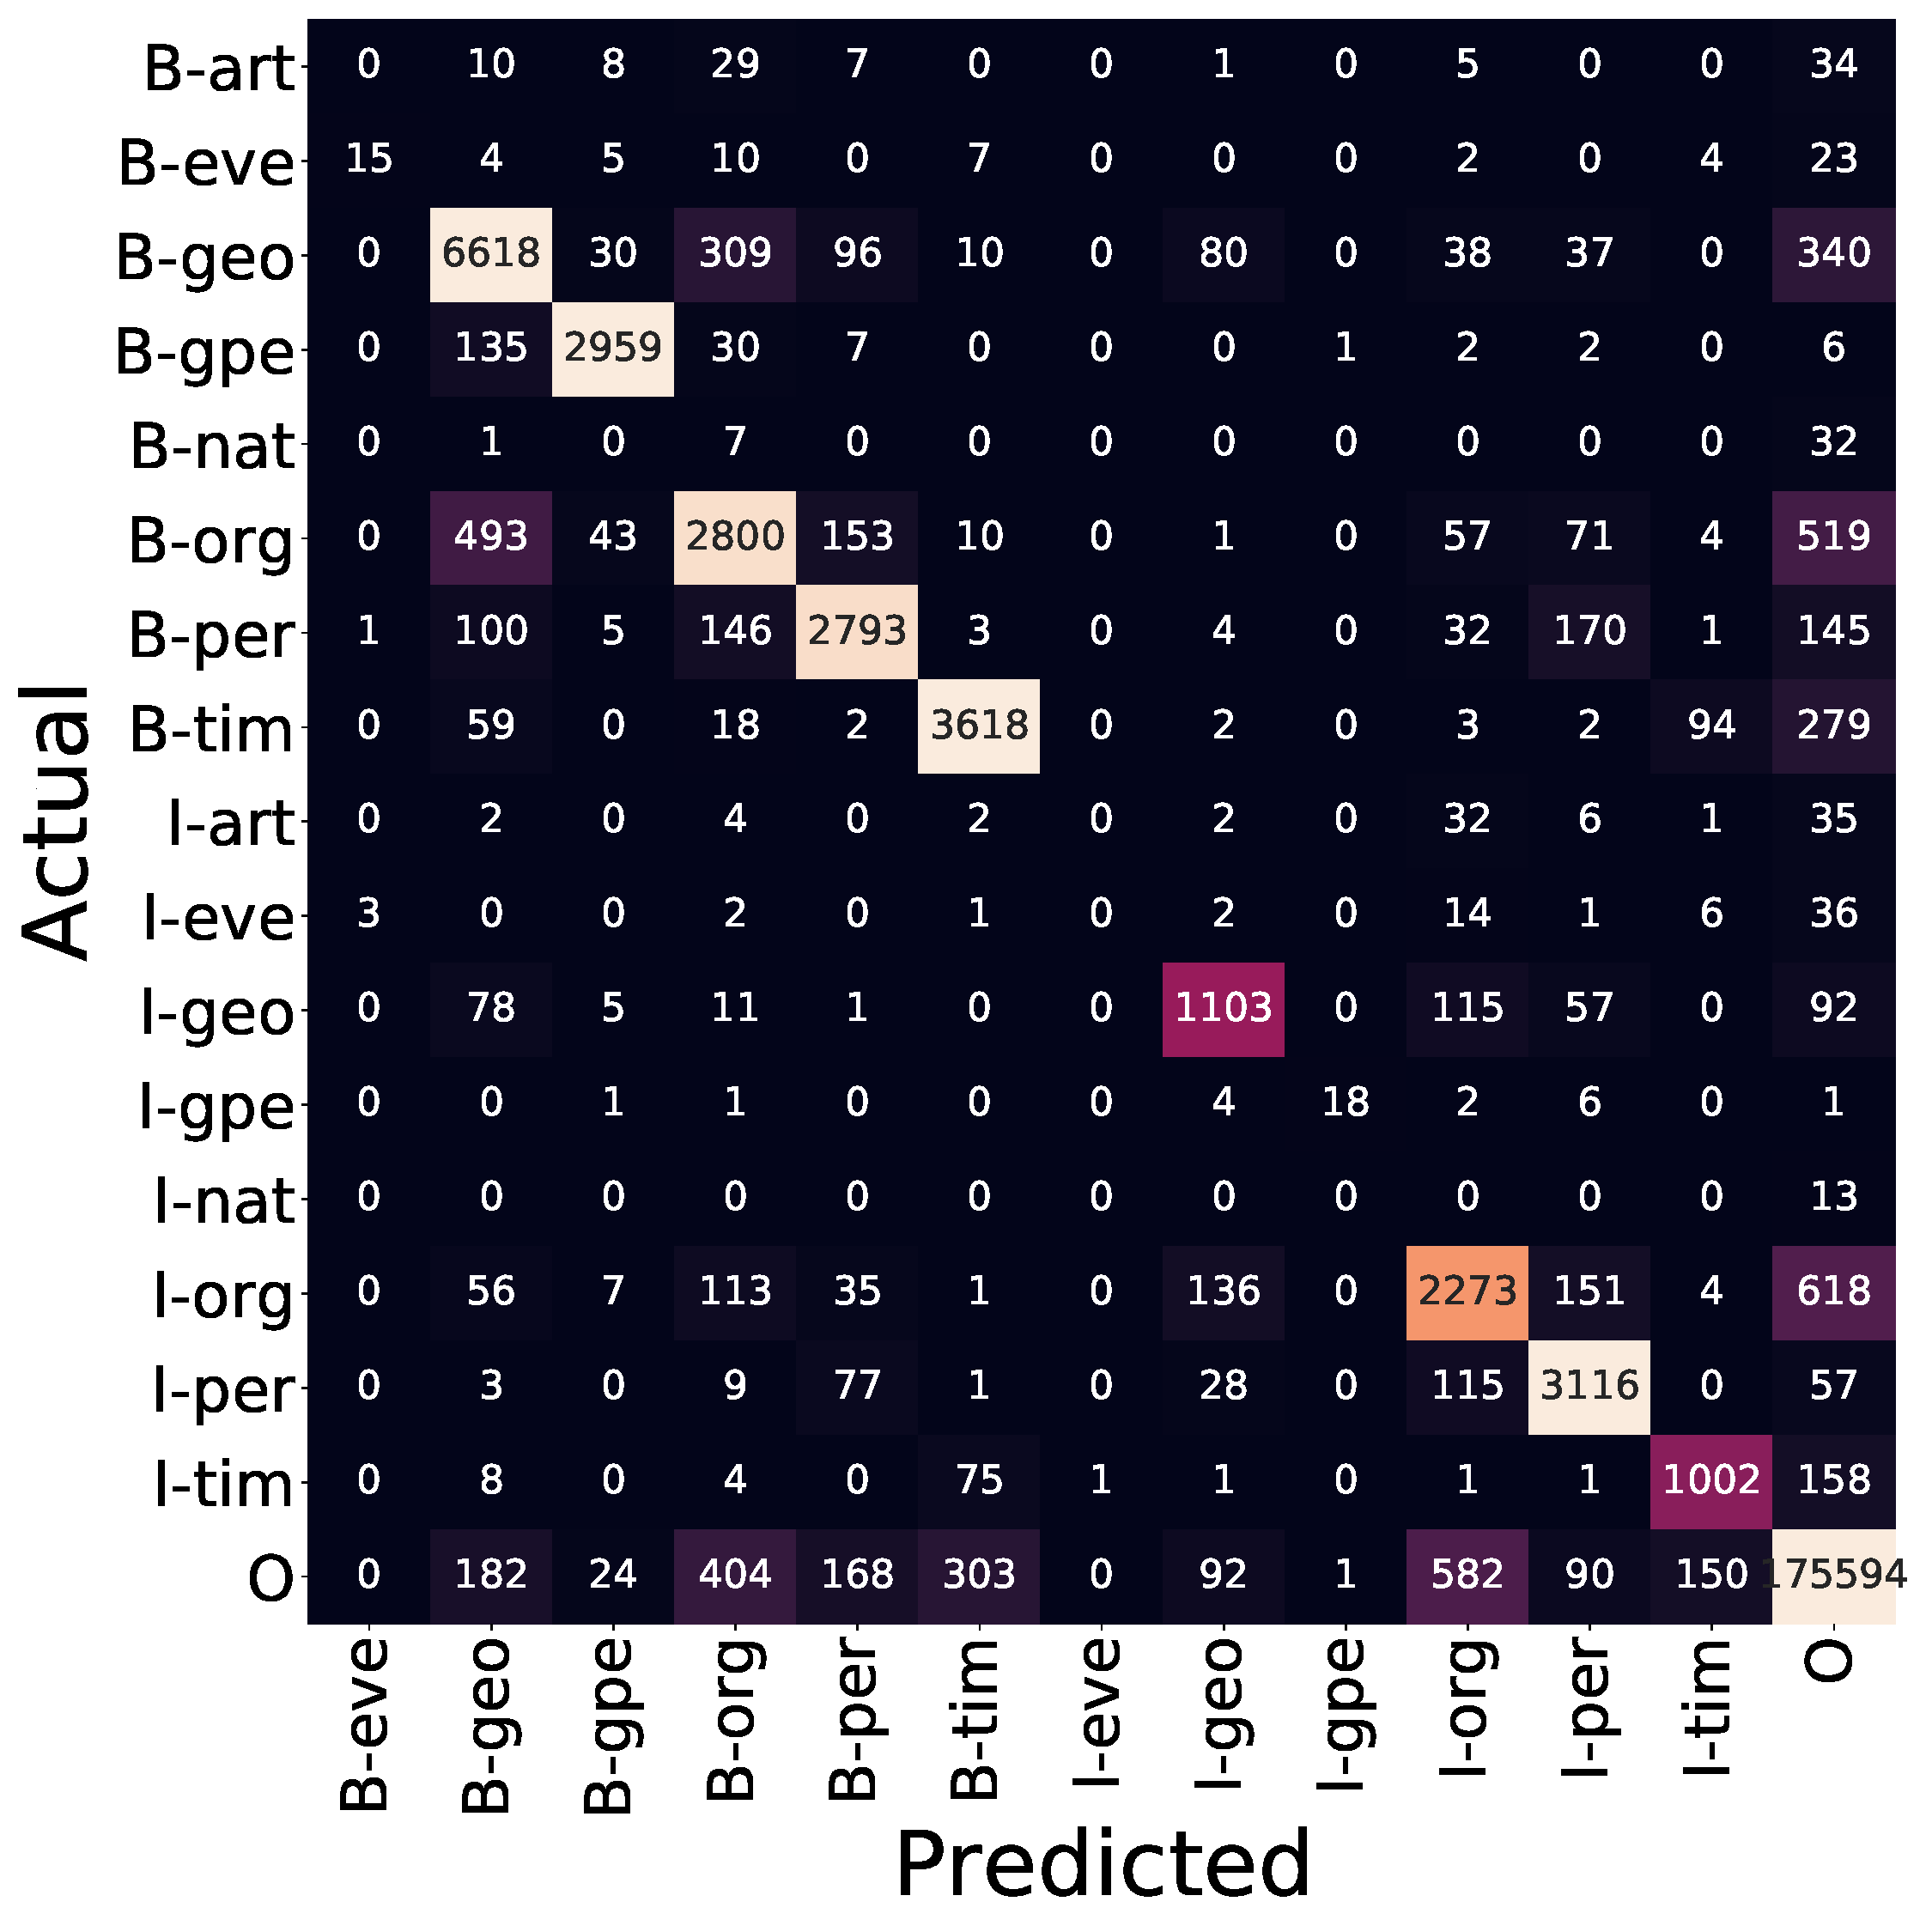
\includegraphics[width=84mm, frame]{../figures/glove_conf_matrix.pdf}
  \end{subfig}
  % figure captions below figure
  \caption{Confusion matrix for the ground truth labels vs the predicted labels using a) Bidirectional LSTM and b) Bidirectional LSTM with GloVe. Notice the increase in number of TP for using the bidirectional LSTM with GloVe over the Bidirectional LSTM model.}
  \label{fig:bilstmconfusion}
\end{figure}

\hfill\\
To further evaluate the model for testing, we measure the metrics in Table.~\ref{tbl:lstm_results}. The recorded metrics using the package seqeval (see Section ~\ref{sec:metrics}) for the prediction of the test. The recorded micro and macro F1 are $0.793$ and $0.547$ respectively. From the table, we notice that the label 'ART' has the lowest measured metrics while the label 'GPE' has the highest measured metrics (see Table.~\ref{tbl:entites} for representation of entities). It is important to notice that the recorded values in Table.~\ref{tbl:lstm_results} is different from the recorded values from Table.~\ref{tbl:results_compare} because we use strict measures here.

\begin{table}
  % Table captions always come *above* the table
  \caption{Strict evaluation of Bidirectional LSTM network. Results might vary very slightly because of the randomness of the model weights initialization.}
  \label{tbl:lstm_results}
  \begin{tabular}{c|c|c|c|c}  
    \hline
    & Precision & Recall & F1 & Support \\\hline
    \verb!ART! & \verb!0.000! &  \verb!0.000! & \verb!0.000! & \verb!94! \\
    \verb!EVE! & \verb!0.812!  & \verb!0.186! & \verb!0.302! & \verb!70! \\
    \verb!GEO! & \verb!0.827!  & \verb!0.854! & \verb!0.841! & \verb!7558! \\
    \verb!GPE! & \verb!0.957!  & \verb!0.932! & \verb!0.944! & \verb!3142! \\
    \verb!NAT! & \verb!0.429!  & \verb!0.075! & \verb!0.128! & \verb!40! \\
    \verb!ORG! & \verb!0.666!  & \verb!0.546! & \verb!0.600! & \verb!4151! \\
    \verb!PER! & \verb!0.751!  & \verb!0.696! & \verb!0.722! & \verb!3400! \\
    \verb!TIM! & \verb!0.861!  & \verb!0.825! & \verb!0.842! & \verb!4077! \\\hline
    \verb!Micro! & \verb!0.815!  & \verb!0.772! & \verb!0.793! & \verb!22532! \\
    \verb!Macro! & \verb!0.663!  & \verb!0.514! & \verb!0.547! & \verb!22532! \\
    \verb!Weighted! & \verb!0.806!  & \verb!0.772! & \verb!0.787! & \verb!22532! \\\hline
  \end{tabular}
\end{table}

\subsection{Bidirectional LSTM with GloVe embedding}
From Table.~\ref{tbl:results_compare}, Bidirectional LSTM with GloVe embedding achieved F1 score of $0.9702$ on training data while the scored F1 scores using test data is $0.9633$. It is noticed from Fig.~\ref{fig:f1_bilstm} that the model converges slightly faster than the bidirectional LSTM. The validation F1 score starts with $0.9564$ and ends with with slight improvement at $0.9609$ after epoch number $10$ while the training score continued to increase slightly from $0.8272$ until it reaches $0.9782$ at epoch number $10$.
\hfill\\
Fig.~\ref{fig:f1_bilstm} shows the precision score achieved by model which starts at $0.9644$ and ends at $0.9632$ on validation data. Despite the change of precision score on training data from $0.8996$ till $0.9809$, validation precision score remains almost constant. The precision score of the test data is $0.9669$.    
\hfill\\
Fig.~\ref{fig:f1_bilstm} shows the recall score of bidirectional LSTM model. The recall scores are $0.9755$ and $0.9587$ and $0.9581$ on training and validation data. The recall of the test data is $0.9598$.
\hfill\\
From the heatmap in the Fig.~\ref{fig:bilstmconfusion}, we noticed that the label "O" label or "other", is also accompanied with most of the errors in the prediction similar to the predictions of bidirectional LSTM model. We noticed that several classes such as "I-tim", "I-per" and "I-gpe" and several other labels were predicted more correct with using bidirectional LSTM with GloVe than using birectional LSTM. However, The number of correct predictions of "O" decrease when using the  birectional LSTM with GloVe.  

\begin{table}
  % Table captions always come *above* the table
  \caption{Part of a random sample from test sentences with prediction and actual labels. The sentence is "The report calls on president bush and congress to urge chinese officials..."}
  \label{tbl:end_results}
  \begin{tabular}{lll}  
    \hline
    Word & Actual & Prediction  \\\hline
    \verb!the! & \verb!O! & \verb!O! \\
    \verb!report! & \verb!O! & \verb!O!  \\
    \verb!calls! & \verb!O! & \verb!O!  \\
    \verb!on! & \verb!O! &  \verb!O! \\
    \verb!president! & \verb!B-per! & \verb!B-per! \\
    \verb!bush! & \verb!I-per! & \verb!I-per! \\
    \verb!and! & \verb!O! & \verb!O!  \\
    \verb!congress! & \verb!B-org! &  \verb!B-org!\\
    \verb!to! & \verb!O! & \verb!O!  \\
    \verb!urge! & \verb!O! & \verb!O! \\
    \verb!chinese! & \verb!B-gpe! & \verb!B-gpe! \\
    \verb!officials! & \verb!O! & \verb!O!  \\\hline
  \end{tabular}
\end{table}

\hfill\\
The Table.~\ref{tbl:results_compare} shows the the recorded metrics of prediction of the test data using strict measures. The recorded micro and macro F1 are $0.810$ and $0.585$ respectively. From the table, we notice that the label 'ART' is never predicted correctly using the strict framework. But in general, the micro F1 is of using Bi-LSTM with GloVe is higher than the one with using Bi-LSTM by margin of $0.02$. Similaly, Bi-LSTM with GloVe recall is higher than the recall of Bi-LSTM by a margin of $0.025$ .
\begin{table}
  % Table captions always come *above* the table
  \caption{Strict evaluation of Bidirectional LSTM with GloVe network. Results might vary very slightly because of the randomness of the model weights initialization}
  \label{tbl:lstm_glove_results}
  \begin{tabular}{c|c|c|c|c}  
    \hline
    & Precision & Recall & F1 & Support \\\hline
    \verb!ART! & \verb!0.000! &  \verb!0.000! & \verb!0.000! & \verb!94! \\
    \verb!EVE! & \verb!0.714!  & \verb!0.214! & \verb!0.330! & \verb!70! \\
    \verb!GEO! & \verb!0.840!  & \verb!0.869! & \verb!0.854! & \verb!7558! \\
    \verb!GPE! & \verb!0.954!  & \verb!0.940! & \verb!0.947! & \verb!3142! \\
    \verb!NAT! & \verb!0.308!  & \verb!0.300! & \verb!0.304! & \verb!40! \\
    \verb!ORG! & \verb!0.668!  & \verb!0.586! & \verb!0.624! & \verb!4151! \\
    \verb!PER! & \verb!0.754!  & \verb!0.749! & \verb!0.752! & \verb!3400! \\
    \verb!TIM! & \verb!0.883!  & \verb!0.851! & \verb!0.867! & \verb!4077! \\\hline
    \verb!Micro! & \verb!0.821!  & \verb!0.799! & \verb!0.810! & \verb!22532! \\
    \verb!Macro! & \verb!0.640!  & \verb!0.564! & \verb!0.585! & \verb!22532! \\
    \verb!Weighted! & \verb!0.814!  & \verb!0.799! & \verb!0.806! & \verb!22532! \\\hline
  \end{tabular}
\end{table}

\section{Discussion}\label{sec:discu}
From the observed results, we notice that bidirectional LSTM with GloVe shows slightly better performance than the simple bidirectional LSTM. This observation is supported using strict and non-strict measures. Strict metrics evaluation of the BiLSTm with GloVe shows improvement by a margin of $0.02$ on the micro F1 score, around $0.025$ on the micro recall score and around $0.005$ on the precision score. These observations indicate that the GloVe model gives a better representation of the words than the simple default embedding layer in the model. 
\hfill\\
We notice that the increase in the metrics in validation curve is small. One possible reason for this observation is that the network already captures the patterns in the features while training just after the first epoch.  
\hfill\\
The two models are facing difficulty to predict the "EVE", "ART" and "NAT" correctly and showed poor prediction results. For example, the precision of both the models for "EVE" tag is high relative to the recall because the increase in number of FN. This means that several entities has been predicted as "EVE" in a wrong way.    
\hfill\\
In this report, we do not make explicit comparison with other related work. There are two reason for that: first reason, it is difficult to compare results given the variance in the used methods and the use of evaluation metrics. For example, Entity Disambiguation systems usually uses a different evaluation metrics that tell about the entities that are found and retrieved correctly from a knowledge base such as Wikipedia within $N$ number of nearest neighbours. Second reason is that the data, to the best of our knowledge, was not pre-splitted strictly into train and test set. So, there are no fixed test set to compare the results. In general, several studies used this data by implementing more advanced models such as the NorNE system that was developed by \citet{Jrgensen2020NorNEAN} that achieved state of the art results on this data. Other models are achieving F1 score of $0.93$ by following the Bidirectional Encoder Representations from Transformers architecture (BERT) by \citet{ DBLP:journals/corr/abs-1810-04805} which is beyond the scope of this report. 
\hfill\\
The data is relatively easy to use for named entity recognition and easy to achieve a relatively better results using simple LSTM networks than applying named entity recognition in other specialized domains. The reason for is that majority of the entities are of the type "B-entity", or unigram for simplicity, where each one of those is considered as one TP in the metrics calculations. Another reason is that the words can be represented easily using GloVe or Word2Vec given that the words are commonly written in articles and general and have less ambiguity. Using more sophisticated pre-trained models such as BERT or ELMo \citep{DBLP:journals/corr/abs-1802-05365} for encoding these words with context embeddings can help even more in boosting our results.

\section{Conclusion}\label{sec:conclusion}
Two LSTM architectures are used to extract entities from the Groningen Meaning Bank (GMB) corpus \citep{Bos2017GMB}. The data in general provides a relatively easy task to solve given that it is from general domain where a model like GloVe can excel. GloVe provides a better representation of the words in the data which is helpful in training the model. Recently, several recent models are built using BERT models which provide an accurate way to encode the word features through combination of word pieces and these models can achieve state of the art results which could be the next step to further develop the results. Also, Further directions and development of the methods are expected to improve the measured metrics on this data by using feature engineering. 

\section{Acknowledgement}\label{sec:akns}
We want to express our gratitude to Prof. Hans Plesser for the guidance and providing detailed feedbacks, encouragement and the help through this study.

% In the acks section, you can thank people for help.
%\ begin{acks}
% We want to express our gratitude to Prof. Hans Plesser for the guidance through this study.
% \end{acks}


%% The next two lines define the bibliography style to be used, and
%% the bibliography file.
\bibliographystyle{ACM-Reference-Format}
\bibliography{biblio_file}

\end{document}
